\chapter{Desarrollo del Relevamiento}
\label{sec.tp2:desarrollo}

En esta sección se detallan las características constructivas de la habitación relevada (compuesta por dos sectores: la
oficina y el depósito), se definen las especificaciones del sistema de iluminación (general y localizado) y se
desarrollan los cálculos normativos para el dimensionamiento de las grillas de medición.

\section{Descripción del Local y Geometría}
\label{sec.tp2:descripcion_local}

El local relevado se encuentra dividido en dos espacios diferenciados de geometría regular: la oficina (área grande) y
el depósito (área chica). El techo de toda la habitación se encuentra a una altura uniforme de $2{,}50\m$ desde el
piso. La reflectancia de las paredes es media-alta (blanco mate) y el suelo es de cerámicos claros.

Las dimensiones geométricas de ambos sectores son:
\begin{itemize}
    \item \textbf{Oficina (Sector Principal):}
    \begin{itemize}
        \item Ancho ($a_{of}$): $3{,}28\m$
        \item Largo ($b_{of}$): $3{,}52\m$
    \end{itemize}
    \item \textbf{Depósito (Sector Secundario):}
    \begin{itemize}
        \item Ancho ($a_{dep}$): $1{,}15\m$
        \item Largo ($b_{dep}$): $1{,}92\m$
    \end{itemize}
    \item \textbf{Alturas de Referencia:}
    \begin{itemize}
        \item Altura total del techo ($H$): $2{,}50\m$
        \item Altura del plano de trabajo ($h_p$): $0{,}80\m$ (altura de los escritorios)
        \item Altura de montaje de luminarias generales ($H_{lum}$): $2{,}50\m$ (montadas directamente al techo)
    \end{itemize}
\end{itemize}

En la oficina se encuentran dos escritorios: un escritorio de trabajo principal de dimensiones extensas ($1{,}88\m \times 0{,}50\m$) ubicado contra la pared izquierda, y un escritorio secundario pequeño de ($1{,}20\m \times 0{,}76\m$) ubicado en la esquina superior derecha.

\section{Especificaciones del Sistema de Iluminación}
\label{sec.tp2:especificaciones_luces}

Todas las fuentes de luz instaladas en los dos sectores corresponden a tecnología LED de temperatura de color blanca fría ($\ge 6000\Kelvin$). El sistema se divide en iluminación general e iluminación localizada:

\subsection{Iluminación General (Techo)}
\begin{itemize}
    \item \textbf{Luminaria General Oficina (P1):} Un ($1$) plafón LED de adosar de $18\W$, luz fría, ubicado en el centro geométrico del cielorraso de la oficina.
    \item \textbf{Luminaria General Depósito (P2):} Un ($1$) plafón LED de adosar de $18\W$, luz fría, ubicado en el centro geométrico del cielorraso del depósito.
\end{itemize}

\subsection{Iluminación Localizada (Escritorios)}
\begin{itemize}
    \item \textbf{Escritorio Largo (Pared Izquierda):} Equipado con una tira LED 5050 monocolor fría de punta a punta ($1{,}88\m$). Presenta una densidad de 3 leds cada $5\cm$ ($60\text{ leds}/\m$, totalizando $113$ leds). Está montada en un perfil de aluminio a $62\cm$ sobre el plano de trabajo (altura respecto al piso $h = 1{,}42\m$). Consumo estimado de $14{,}4\W/\m$ (potencia de la tira $\approx 27\W$) y un flujo total de $\approx 1800\lumen$.
    \item \textbf{Escritorio Chico (Esquina Superior Derecha):} Equipado con una luminaria de mesa regulable LED, luz fría, con un flujo luminoso máximo de $700\lumen$ y una potencia aproximada de $18\W$, montada de forma centrada a una altura de $65\cm$ sobre el plano de trabajo (altura respecto al piso $h = 1{,}45\m$).
\end{itemize}

\section{Cálculo del Índice del Local y Puntos de Medición}
\label{sec.tp2:calculo_grilla}

La altura de montaje de las luminarias generales respecto al plano de trabajo es:
\begin{equation}
    h_m = H_{lum} - h_p = 2{,}50\m - 0{,}80\m = 1{,}70\m
\end{equation}

Se realizan los cálculos del Índice de Local ($k$) y de la cantidad de puntos de medición mínimos ($N$) de forma independiente para cada área:

\subsection{Área de Oficina (Grande)}
\begin{equation}
    k_{oficina} = \frac{3{,}28\m \cdot 3{,}52\m}{1{,}70\m \cdot (3{,}28\m + 3{,}52\m)} = \frac{11{,}5456}{11{,}56} \approx 1{,}00
\end{equation}
Dado que $k \le 1$, el índice redondeado es $k_{red} = 1$. La cantidad mínima de puntos de medición se calcula como:
\begin{equation}
    N_{oficina} = (1 + 2)^2 = 9\text{ puntos (grilla de } 3 \times 3\text{)}
\end{equation}
Las celdas resultantes de la división tienen dimensiones de $1{,}173\m$ de largo por $1{,}093\m$ de ancho.

\subsection{Área de Depósito (Chico)}
\begin{equation}
    k_{deposito} = \frac{1{,}15\m \cdot 1{,}92\m}{1{,}70\m \cdot (1{,}15\m + 1{,}92\m)} = \frac{2{,}208}{5{,}219} \approx 0{,}42
\end{equation}
Dado que $k \le 1$, el índice redondeado es $k_{red} = 1$. El número mínimo de puntos de medición general es:
\begin{equation}
    N_{deposito} = (1 + 2)^2 = 9\text{ puntos (grilla de } 3 \times 3\text{)}
\end{equation}
Las celdas resultantes de la división tienen dimensiones de $0{,}64\m$ de largo por $0{,}383\m$ de ancho.

\subsection{Puntos de Iluminación Localizada}
Para verificar el aporte lumínico localizado, se realizaron mediciones directas sobre los escritorios:
\begin{itemize}
    \item En el escritorio largo se determinan 3 puntos equidistantes distribuidos a lo largo del mismo ($E_{L1}, E_{L2}, E_{L3}$).
    \item En el escritorio chico se determina 1 punto centrado en el área de trabajo ($E_{C1}$).
\end{itemize}

\section{Croquis e Implantación del Local}
\label{sec.tp2:croquis}

El croquis detallado de planta de la habitación, con la delimitación de ambos sectores (oficina y depósito), la ubicación de los escritorios, las luminarias generales y localizadas, y la grilla de medición resultante, se representa en la Figura~\ref{fig.tp2:croquis_habitacion}.

\begin{figure}[!ht]
    \centering
    \begin{tikzpicture}[scale=2.0, >=latex]
    % === ESTILOS ===
    \tikzstyle{wall} = [black, line width=2.0pt]
    \tikzstyle{desk} = [pattern=north west lines, pattern color=gray!30, draw=gray, line width=0.8pt]
    \tikzstyle{window} = [blue!80!black, line width=2.5pt, double, double distance=1.5pt]
    \tikzstyle{cota} = [gray!80!black, thin, <->]
    \tikzstyle{cotaline} = [gray!40, thin]
    \tikzstyle{gridline} = [blue!15, dashed, ultra thin]

    % === INDICACIÓN DEL SUR (A LA IZQUIERDA DEL CROQUIS) ===
    \draw[thick, ->] (-0.5, 1.64) -- (-0.9, 1.64) node[left, font=\bfseries\small] {SUR};

    % === DIBUJO DE PISO Y PAREDES ===
    \fill[gray!2] (0,0) -- (0,3.28) -- (3.52,3.28) -- (3.52,0) -- cycle;
    \fill[gray!4] (0.54,3.28) -- (0.54,5.32) -- (1.69,5.32) -- (1.69,3.28) -- cycle;

    % Paredes externas
    \draw[wall] (0,0) -- (0,1.88) -- (0.34, 1.88) -- (0.34, 2.25) -- (0, 2.25) -- (0, 3.28) 
                -- (0.54, 3.28) -- (0.54, 5.32) -- (1.69, 5.32) -- (1.69, 3.28) 
                -- (3.52, 3.28) -- (3.52, 0) -- (0,0);

    % Ventanas
    \draw[window] (.65, 0) -- ++(.62, 0);
    \draw[window] (3.52, .7) -- ++(0, 1.88);

    % === MUEBLES (ESCRITORIOS) ===
    \draw[desk] (0, 0) rectangle (0.5, 1.88);
    \draw[desk] (3.52, 3.28) rectangle (2.76, 2.08);

    % === GRILLES DE MEDICIÓN GENERAL (LÍNEAS DE TRAZOS) ===
    \foreach \x in {1.173, 2.346} {
        \draw[gridline] (\x, 0) -- (\x, 3.28);
    }
    \foreach \y in {1.093, 2.186} {
        \draw[gridline] (0, \y) -- (3.52, \y);
    }

    \foreach \x in {0.923, 1.306} {
        \draw[gridline] (\x, 3.40) -- (\x, 5.32);
    }
    \foreach \y in {4.04, 4.68} {
        \draw[gridline] (0.54, \y) -- (1.69, \y);
    }

    % Puntos de Iluminación Localizada - Cruces Rojas
    \foreach \py/\pnum in {0.31/1, 0.94/2, 1.57/3} {
        \draw[red!85!black, thick] (0.25-0.05, \py) -- (0.25+0.05, \py);
        \draw[red!85!black, thick] (0.25, \py-0.05) -- (0.25, \py+0.05);
        \node[right, scale=0.5, red!70!black] at (0.27, \py) {$E_{L\pnum}$};
    }
    \draw[red!85!black, thick] (3.14-0.05, 2.68) -- (3.14+0.05, 2.68);
    \draw[red!85!black, thick] (3.14, 2.68-0.05) -- (3.14, 2.68+0.05);
    \node[above left, scale=0.5, red!70!black] at (3.12, 2.68) {$E_{C1}$};

    % === LUMINARIAS (SIN TEXTOS DE ACLARACIÓN ADENTRO) ===
    % 1. Plafón General Oficina (Centrado en Oficina: 1.76, 1.64)
    \draw[fill=cyan!10, draw=cyan!80!black, double, thick] (1.76, 1.64) circle (0.10);
    \draw[cyan!80!black, thin] (1.76-0.10, 1.64) -- (1.76+0.10, 1.64);
    \draw[cyan!80!black, thin] (1.76, 1.64-0.10) -- (1.76, 1.64+0.10);

    % 2. Plafón General Depósito (Centrado en Depósito: 1.115, 4.36)
    \draw[fill=cyan!10, draw=cyan!80!black, double, thick] (1.115, 4.36) circle (0.10);
    \draw[cyan!80!black, thin] (1.115-0.10, 4.36) -- (1.115+0.10, 4.36);
    \draw[cyan!80!black, thin] (1.115, 4.36-0.10) -- (1.115, 4.36+0.10);

    % 3. Tira LED Escritorio Largo (x=0.25, de y=0.1 a y=1.78)
    \draw[yellow!80!orange, line width=2.2pt, cap=round] (0.25, 0.1) -- (0.25, 1.78);

    % 4. Luminaria Regulable Escritorio Chico (Centrado en Escritorio Chico: 3.14, 2.68)
    \draw[fill=yellow!20, draw=yellow!80!orange, thick] (3.14, 2.68) circle (0.07);
    \draw[yellow!80!orange, fill=yellow!80!orange] (3.14, 2.68) circle (0.02);


    % === PUNTOS DE MEDICIÓN ===
    % Puntos Oficina (E1 a E9) - Círculos Naranjas
    \def\ox{3.52/3}
    \def\oy{3.28/3}
    \foreach \ix in {1,2,3} {
        \foreach \iy in {1,2,3} {
            \pgfmathsetmacro{\px}{(\ix - 0.5) * \ox}
            \pgfmathsetmacro{\py}{(\iy - 0.5) * \oy}
            \pgfmathsetmacro{\pnum}{int((\iy - 1) * 3 + \ix)}
            \fill[orange!85!black] (\px, \py) circle (0.04);
            \node[below, scale=0.8, orange!65!black] at (\px, \py) {$E_{\pnum}$};
        }
    }

    % Puntos Depósito (E10 a E18) - Círculos Naranjas
    \def\dx{1.15/3}
    \def\dy{1.92/3}
    \foreach \ix in {1,2,3} {
        \foreach \iy in {1,2,3} {
            \pgfmathsetmacro{\px}{0.54 + (\ix - 0.5) * \dx}
            \pgfmathsetmacro{\py}{3.40 + (\iy - 0.5) * \dy}
            \pgfmathsetmacro{\pnum}{int(9 + (\iy - 1) * 3 + \ix)}
            \fill[orange!85!black] (\px, \py) circle (0.04);
            \node[below, scale=0.8, orange!65!black] at (\px, \py) {$E_{\pnum}$};
        }
    }

    % === TEXTOS / ROTULACIÓN DE AREAS ===
    \node[scale=0.8, font=\bfseries, text=gray!70] at (1.76, 1) {OFICINA};
    \node[scale=0.8, font=\bfseries, text=gray!70] at (1.115, 4.65) {DEPÓSITO};

    % === COTAS ===
    \draw[cotaline] (0,0) -- (0,-0.25);
    \draw[cotaline] (3.52,0) -- (3.52,-0.25);
    \draw[cota] (0,-0.20) -- (3.52,-0.20) node[midway, fill=white, scale=0.7] {$3{,}52\m$};

    \draw[cotaline] (3.52,0) -- (3.77,0);
    \draw[cotaline] (3.52,3.28) -- (3.77,3.28);
    \draw[cota] (3.72,0) -- (3.72,3.28) node[midway, rotate=-90, fill=white, scale=0.7] {$3{,}28\m$};

    \draw[cotaline] (0.54,5.32) -- (0.54,5.57);
    \draw[cotaline] (1.69,5.32) -- (1.69,5.57);
    \draw[cota] (0.54,5.52) -- (1.69,5.52) node[midway, fill=white, scale=0.7] {$1{,}15\m$};

    \draw[cotaline] (0.54,3.28) -- (0.29,3.28);
    \draw[cotaline] (0.54,5.32) -- (0.29,5.32);
    \draw[cota] (0.34,3.28) -- (0.34,5.32) node[midway, rotate=90, fill=white, scale=0.7] {$1{,}92\m$};

    \draw[cotaline] (0,1.88) -- (0.45,1.88);
    \draw[cotaline] (0,2.25) -- (0.45,2.25);
    \draw[cota] (0.40,1.88) -- (0.40,2.25) node[midway, right, scale=0.55] {$0{,}37\m$};
    
    \draw[cotaline] (0,1.88) -- (0,2.35);
    \draw[cotaline] (0.34,1.88) -- (0.34,2.35);
    \draw[cota] (0,2.30) -- (0.34,2.30) node[midway, above, scale=0.55] {$0{,}34\m$};

    % === LISTA DE REFERENCIAS AL COSTADO (SIN LÍNEA PUNTEADA NI DE PARED) ===
    \node[anchor=west] at (4.0, 4.8) {\textbf{Referencias:}};
    
    % Plafón LED General
    \draw[fill=cyan!10, draw=cyan!80!black, double, thick] (4.2, 4.4) circle (0.08);
    \draw[cyan!80!black, thin] (4.2-0.08, 4.4) -- (4.2+0.08, 4.4);
    \draw[cyan!80!black, thin] (4.2, 4.4-0.08) -- (4.2, 4.4+0.08);
    \node[anchor=west, scale=0.7] at (4.5, 4.4) {Plafón LED General (18W)};
    
    % Tira LED Localizada
    \draw[yellow!80!orange, line width=2.5pt, cap=round] (4.1, 3.9) -- (4.3, 3.9);
    \node[anchor=west, scale=0.7] at (4.5, 3.9) {Tira LED Localizada (5050)};
    
    % Luminaria Focalizada
    \draw[fill=yellow!20, draw=yellow!80!orange, thick] (4.2, 3.4) circle (0.06);
    \draw[yellow!80!orange, fill=yellow!80!orange] (4.2, 3.4) circle (0.02);
    \node[anchor=west, scale=0.7] at (4.5, 3.4) {Luz Focalizada Escritorio (700lm)};
    
    % Punto de Medición General
    \fill[orange!85!black] (4.2, 2.9) circle (0.04);
    \node[anchor=west, scale=0.7] at (4.5, 2.9) {Punto de Medición General ($E_i$)};
    
    % Punto de Medición Localizado
    \draw[red!85!black, thick] (4.2-0.04, 2.4) -- (4.2+0.04, 2.4);
    \draw[red!85!black, thick] (4.2, 2.4-0.04) -- (4.2, 2.4+0.04);
    \node[anchor=west, scale=0.7] at (4.5, 2.4) {Punto Medición Localizado ($E_{Lx}, E_{Cx}$)};

\end{tikzpicture}

    \caption{Croquis de planta en escala.}
    \label{fig.tp2:croquis_habitacion}
\end{figure}

\section{Relevamiento Fotográfico del Ambiente}
\label{sec.tp2:fotos_ambiente}

En las Figuras~\ref{fig.tp2:foto_oficina} y \ref{fig.tp2:foto_deposito} se presentan las fotografías reales tomadas en el local durante las mediciones para constatar el estado general de los sectores, de los puestos y de las luminarias.

\begin{figure}[!ht]
    \centering
    \begin{subfigure}[t]{0.48\textwidth}
        \centering
        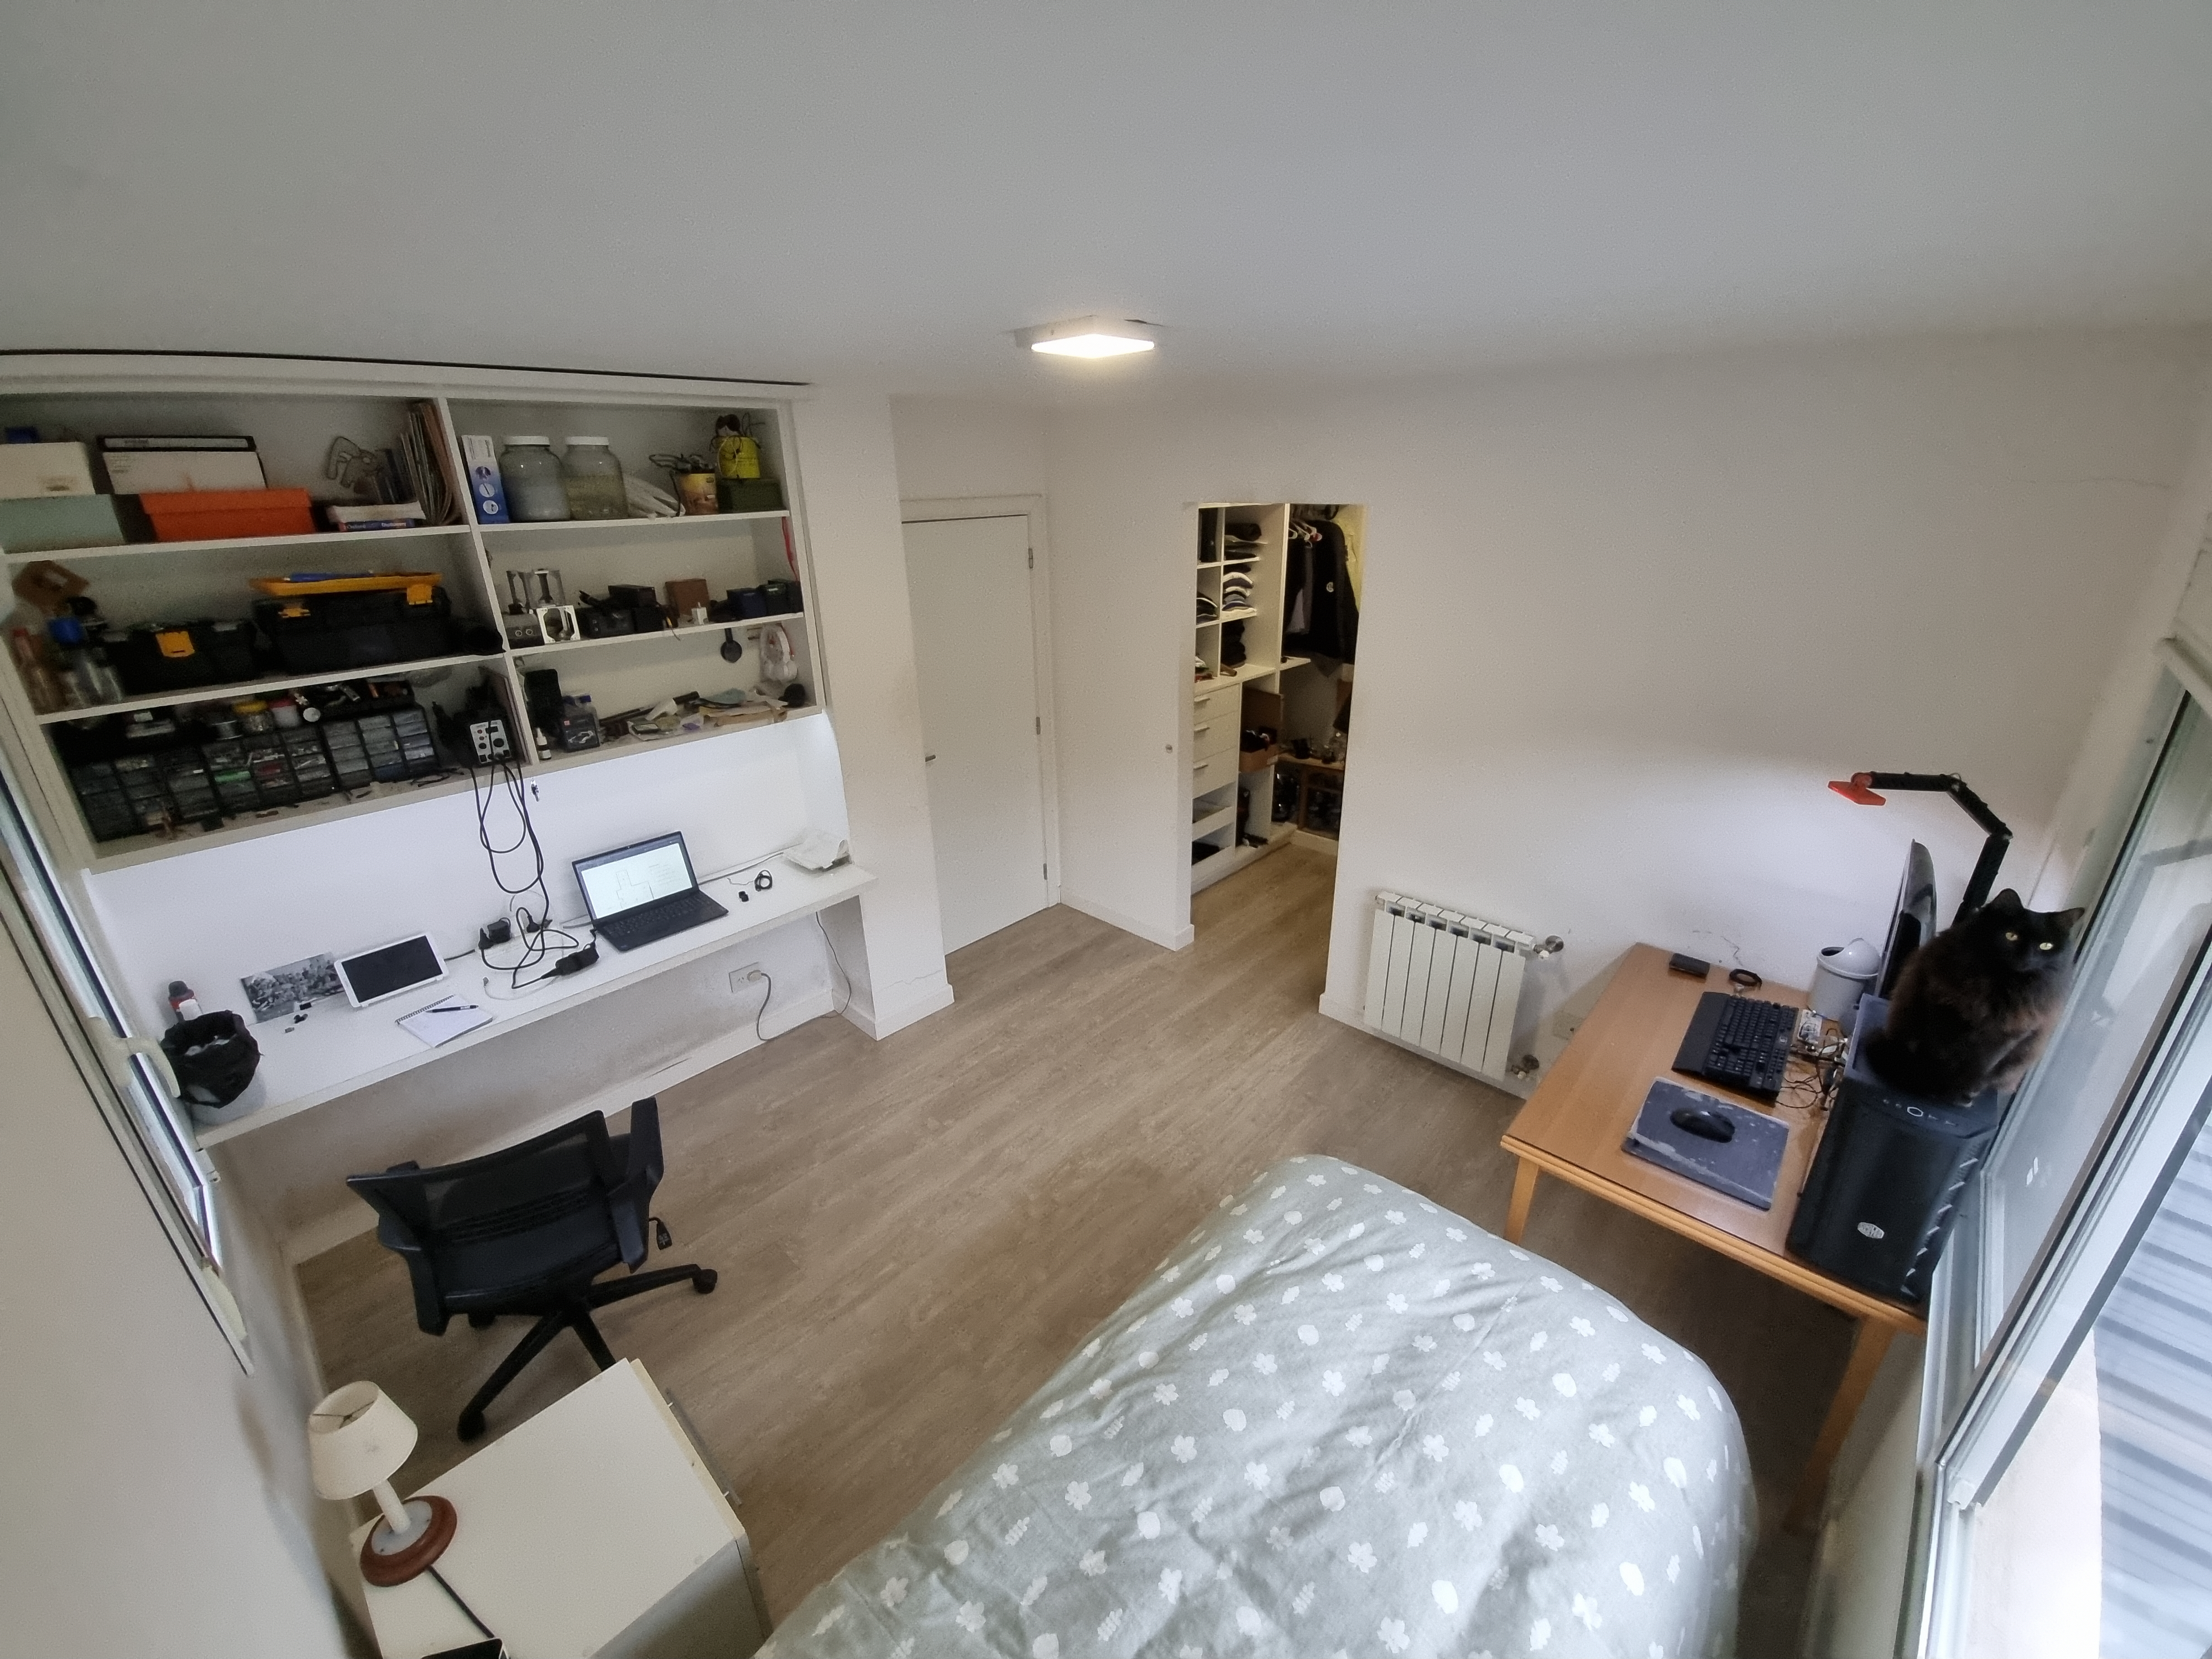
\includegraphics[width=\textwidth]{pictures/foto_oficina.jpg}
        \caption{Fotografía de la oficina técnica.}
        \label{fig.tp2:foto_oficina}
    \end{subfigure}
    \hfill
    \begin{subfigure}[t]{0.48\textwidth}
        \centering
        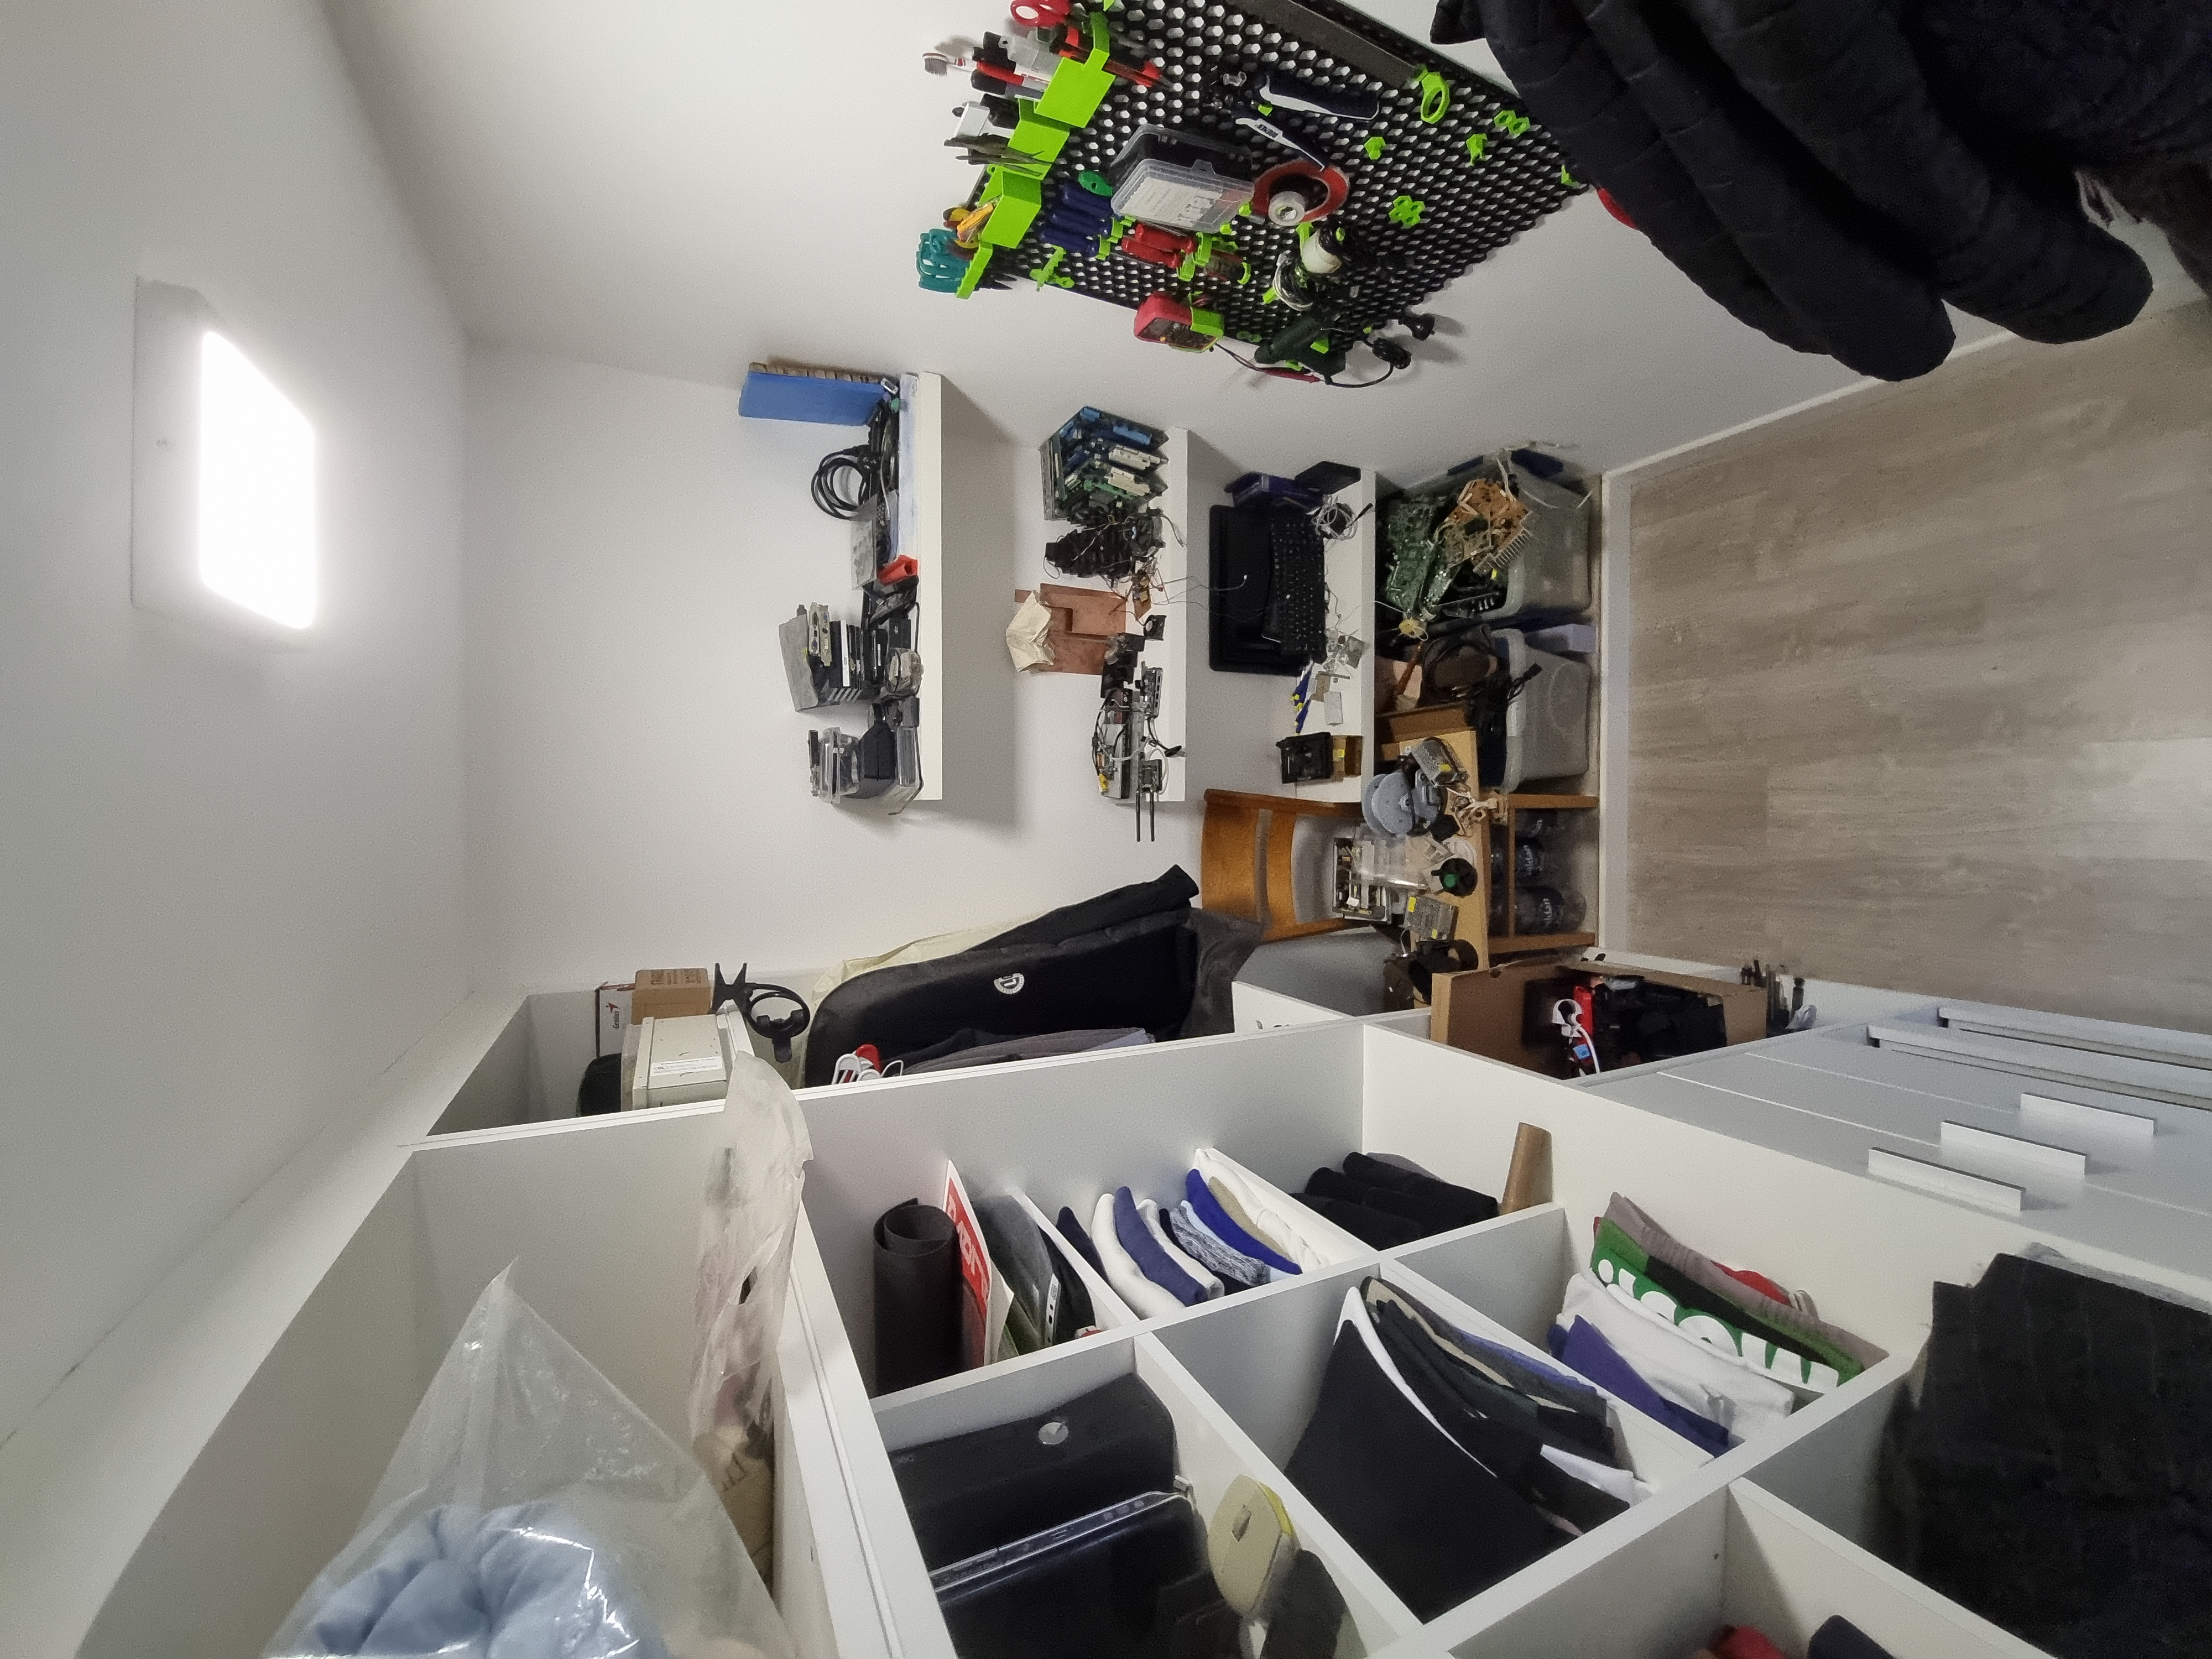
\includegraphics[width=\textwidth]{pictures/foto_deposito.jpg}
        \caption{Fotografía del depósito.}
        \label{fig.tp2:foto_deposito}
    \end{subfigure}
    \caption{Relevamiento fotográfico de los sectores de la habitación.}
    \label{fig.tp2:fotos_relevamiento}
\end{figure}
